% -*- root: ../main.tex -*-
%!TEX root = ../main.tex
% vim:textwidth=120 fo=cqt

\frontmatter
\pagenumbering{arabic} % Imperial College requirement is that all pages must be in continuous arabic numbering
\graphicspath{{frontmatter/figures/}}


% Title page
% \pdfbookmark[chapter]{Title Page}{coverpage}

\includepdf[link, linkname=coverpage, addtotoc={1,chapter,0,Title Page,coverpage}, pages=-, pagecommand={\thispagestyle{plain}}]{frontmatter/coverpage.pdf}

% -*- root: ../main.tex -*-
%!TEX root = ../main.tex
% vim:textwidth=80 fo=cqt

\cleardoublepage

\newpage\null\thispagestyle{plain}\AddToShipoutPictureBG*{%
    \put(0,545){%
        \transparent{0.4}
\includegraphics[width=\paperwidth,keepaspectratio]{wordcloud}%
    }%
}
\vfill
% \begin{minipage}[t]{105mm}
\parbox{130mm}{
    \doublespacing
    \noindent The professional biographical profile of this thesis author is available online at
    \url{https://www.linkedin.com/in/krishnakumargopalakrishnan/}
}
% \end{minipage}
% \begin{varwidth}[t]{10mm}
    \blackurl
    \qrcode[height=0.5in]{https://www.linkedin.com/in/krishnakumargopalakrishnan/}
    \regularurl
% \end{varwidth}
\newpage


% -*- root: ../main.tex -*-
%!TEX root = ../main.tex
% vim:textwidth=80 fo=cqt

% \pdfbookmark[chapter]{Originality \& Copyright Declarations}{} 

\chapter*{Declaration of Originality \hfill}\label{ch:originality}
\addcontentsline{toc}{chapter}{Declaration of Originality and Copyright}

\vspace*{-1.0cm}

I declare  that the material presented  in this thesis  is the result of  my own
research except  for specific portions wherein  contributions from collaborators
are acknowledged. Throughout this thesis, references are made to other published
works and  these have been appropriately  cited. The material contained  in this
thesis has  not been  submitted, either  in whole or  in part,  for a  degree at
Imperial College London or any other university.\\[-3em]

\begin{flushright}
        \begin{tabular}{@{}p{.4in}p{2.1in}@{}}
            % & 
\includegraphics[angle=-5,width=0.25\textwidth]{black_ink_sign_from_jpg}\\[-2em]
            % Signed: & \hrulefill \\
                    & \phantom{Krishnakumar Gopalakrishnan} \\
                    & Krishnakumar Gopalakrishnan \\
                    & October 02, 2018\\
                    & London, United Kingdom \\
        \end{tabular}
\end{flushright}

{\let\clearpage\relax \chapter*{Declaration of Copyright\hfill}}

\vspace*{-1cm}

\noindent
\begin{minipage}[b]{0.3275\textwidth}
    % https://www.imperial.ac.uk/research-and-innovation/support-for-staff/scholarly-communication/open-access/spiral/licences-and-policies/
    % newer link % https://www.imperial.ac.uk/research-and-innovation/support-for-staff/scholarly-communication/open-access/theses/selecting-a-creative-commons-licence/
    \noindent \raggedright 
\includegraphics[width=\linewidth]{doclicense-CC-by-nc-nd.pdf}
\end{minipage}
\hfill
\hspace*{0.0225\textwidth}
\begin{minipage}[b]{0.65\textwidth}
    The    copyright    of    this     thesis    rests    with    the    author.
    Unless   otherwise    indicated,   its    contents   are    licensed   under
    a   \href{https://creativecommons.org/licenses/by-nc-nd/4.0/}{\mbox{Creative
    Commons}   Attribution-NonCommercial-NoDerivatives  4.0   International  (CC
    BY-NC-ND 4.0) Licence}.
\end{minipage}

\noindent Under this licence, you may  copy and redistribute the material in any
medium or format on the condition that: you credit the author, do not use it for
commercial purposes  and do not distribute  modified versions of the  work. When
reusing or sharing this work, ensure you  make the licence terms clear to others
by naming  the licence and linking  to the licence text.  Please seek permission
from the copyright  holder for uses of  this work that are not  included in this
licence or permitted under UK Copyright Law.

\vfill



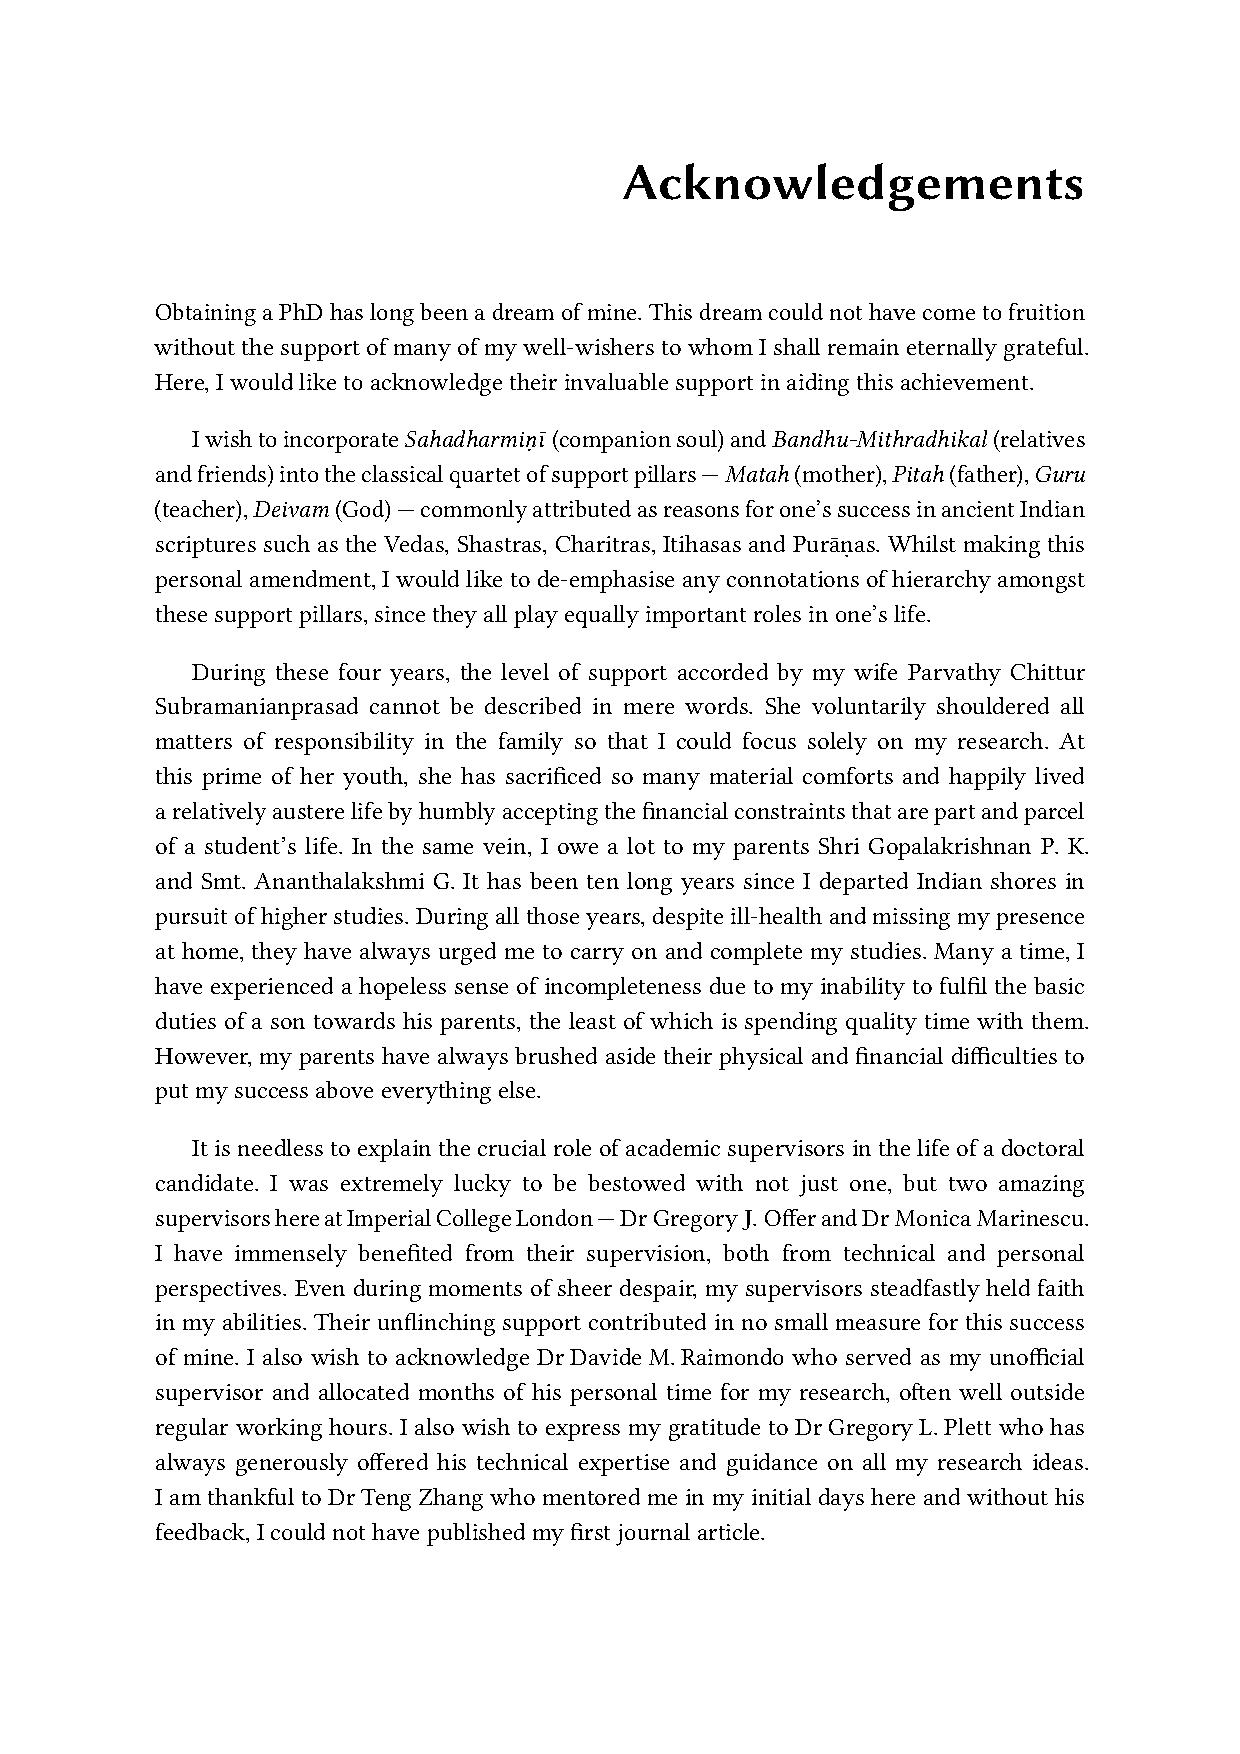
\includepdf[link, linkname=acknowledgements, addtotoc={1,chapter,0,Acknowledgements,acknowledgements}, pages=-,
pagecommand={\thispagestyle{plain}}]{frontmatter/acknowledgements.pdf}
% -*- root: ../main.tex -*-
%!TEX root = ../main.tex
% vim:textwidth=80 fo=cqt

% \afterpage{\null\thispagestyle{plain}\newpage}

\chapter{Dedication\hfill}
% \addcontentsline{toc}{chapter}{Dedication}
\pagecolor{cornsilk}\afterpage{\nopagecolor}

\begingroup
\eachpageornament

\begin{minipage}{\textwidth}
    \vspace*{-2cm}
    \textcolor{black}{\heartpar{To my dear wife, \mbox{Parvathy C.S.}\ and my parents,
            \mbox{Gopalakrishnan P.K.} \& \mbox{Ananthalakshmi G}. The sacrifices that you all made for
            my success is immeasurable and no amount of words shall convey my sheer
    gratitude. I am forever in your debt for your unconditional love. }}

    \vfill
    \centering
    % 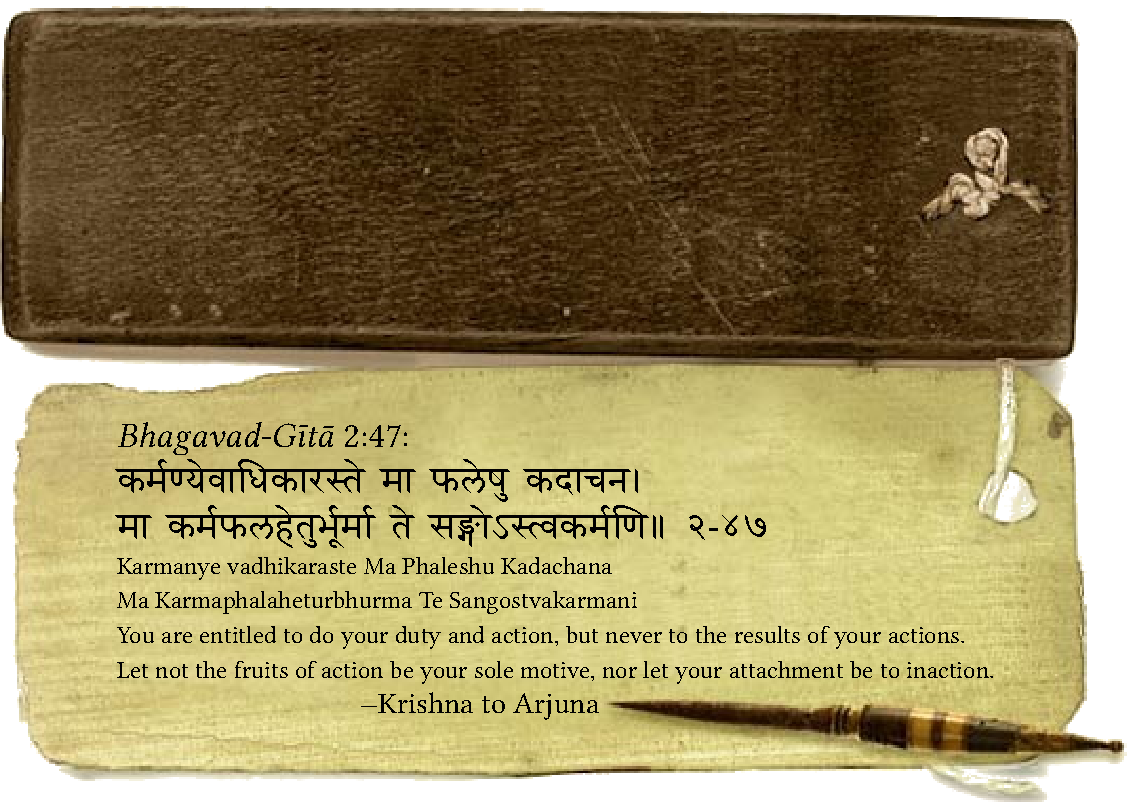
\includegraphics[width=0.85\textwidth]{narayam_sanskrit.png}
    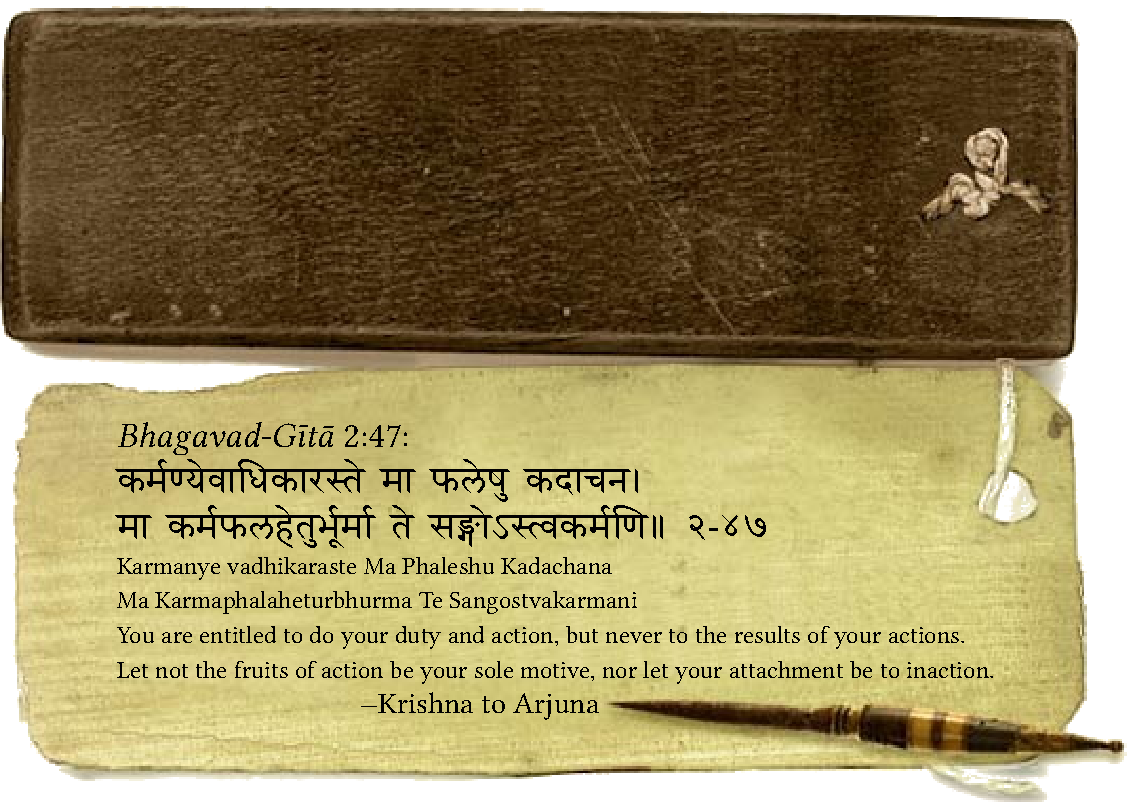
\includegraphics[width=0.85\textwidth]{narayam_sanskrit.pdf}
    \flushright{\scriptsize The image `Thaliyola.jpg' (on which the Gita verse
    is overlaid by this thesis author) was sourced from Wikimedia Commons and is licensed CC-BY-SA 2.5}

    % \pdfbookmark[chapter]{Dedication}{dedication}
\end{minipage}
\endgroup


\setstretch{1.348361657291667}   % golden-ratio stretch (1.2 x 1.348 = 1.618)
% Thesis Abstract -----------------------------------------------------

%\begin{abstractslong}    %uncommenting this line, gives a different abstract heading
\begin{abstracts}        %this creates the heading for the abstract page
\addcontentsline{toc}{chapter}{Abstract}
Put your abstract here...

\end{abstracts}



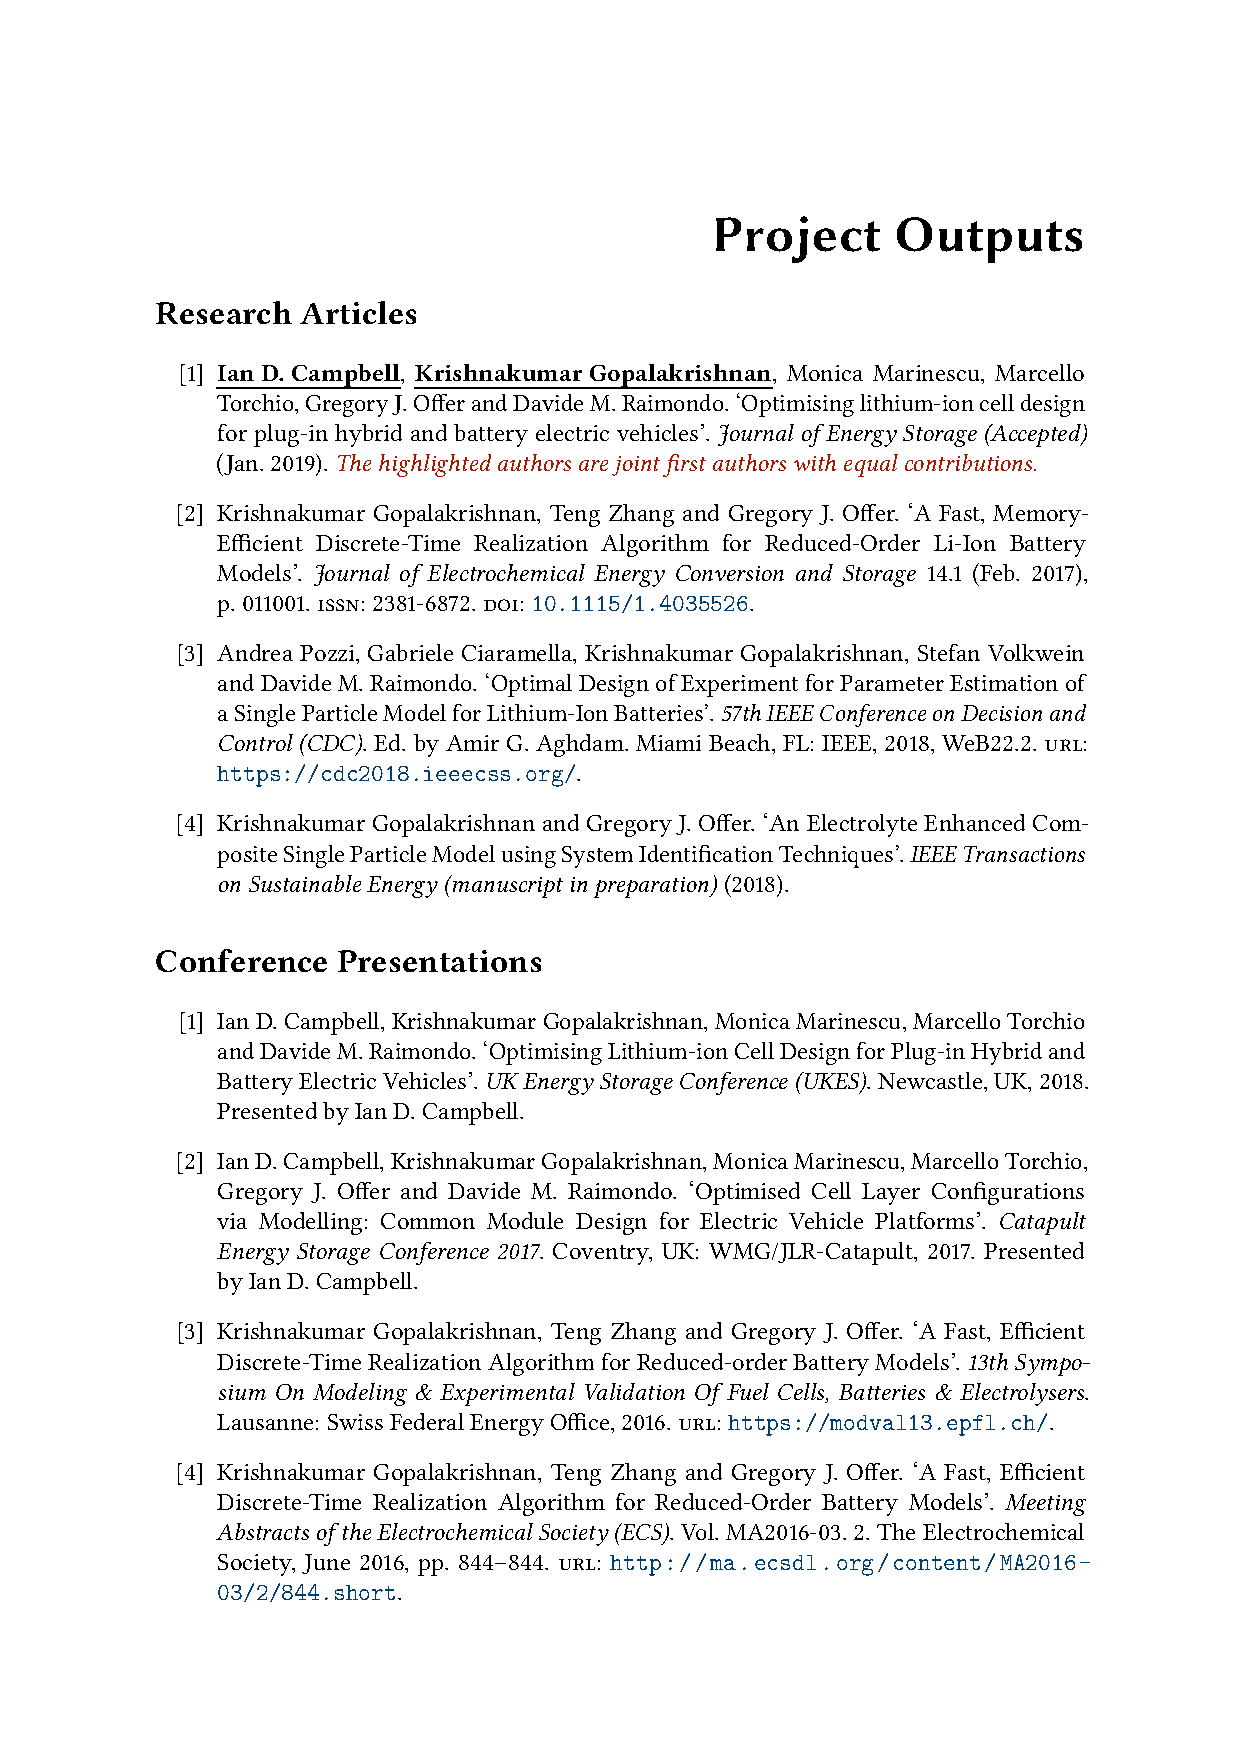
\includepdf[link, linkname=projectoutputs, addtotoc={1,chapter,0,Project outputs,projectoutputs}, pages=-, pagecommand={\thispagestyle{plain}}]{frontmatter/project_outputs.pdf}

%: ----------------- Table of contents/lof/lot/loa etc. ------------------------
\renewcommand{\baselinestretch}{0.3}\normalsize % for toc
\cleardoublepage
\glsunsetall
\microtypesetup{protrusion=false} % disables protrusion locally in the document for typesetting of toc-type matter
\pdfbookmark[chapter]{\contentsname}{toc} % \pdfbookmark[<level>]{<title>}{<dest>} with bookmark package. https://tex.stackexchange.com/questions/65544/how-to-link-table-of-contents-in-thesis-pdf
\tableofcontents
\cleardoublepage
\setstretch{1.1} % for lof
\listoffigures
\cleardoublepage
\onehalfspacing  % for lot
\listoftables
\cleardoublepage
% https://tex.stackexchange.com/questions/69184/remove-blank-page-between-list-of-figures-and-list-of-tables
{\listofalgorithms \let\clearpage\relax \addcontentsline{toc}{chapter}{List of Algorithms} \begingroup \tcblistof[\chapter*]{mypyg}{List of Program Code} \endgroup \addcontentsline{toc}{chapter}{List of Program Code}} % All of this is a hack and must be investigated properly when reusing these macros for other similar long documents
\microtypesetup{protrusion=true} % re-enables protrusion
\glsresetall
%:------------------ End of table of contents/lof/lot/loa etc.----------

% \setstretch{1.0} % for acronyms
\setstretch{1.025}
{%
\setlength{\glsdescwidth}{0.99\textwidth}
\printunsrtglossary[type=acronym, title={List of Acronyms}, nonumberlist, style=super]\label{ch:glossary}
}%
\renewcommand{\baselinestretch}{0.3}\normalsize
\printunsrtglossary[type=symbols, title={List of Symbols}, style=alttreegroup]\label{ch:symbols}


